% =========================================================================
% SciPost LaTeX template (structure of the 2024-07 skeleton)
% =========================================================================
\documentclass[submission, Phys]{SciPost}

% Prevent all line breaks in inline equations.
\binoppenalty=10000
\relpenalty=10000

\hypersetup{
    colorlinks,
    linkcolor={red!50!black},
    citecolor={blue!50!black},
    urlcolor={blue!80!black}
}

\usepackage[bitstream-charter]{mathdesign}
\urlstyle{same}

% Fix \cal and \mathcal characters look (so it's not the same as \mathscr)
\DeclareSymbolFont{usualmathcal}{OMS}{cmsy}{m}{n}
\DeclareSymbolFontAlphabet{\mathcal}{usualmathcal}

\fancypagestyle{SPstyle}{
\fancyhf{}
\lhead{\colorbox{scipostdeepblue}{\bf \color{white} ~SciPost Physics }}
\rhead{{\bf \color{scipostdeepblue} ~Submission }}
\renewcommand{\headrulewidth}{1pt}
\fancyfoot[C]{\textbf{\thepage}}
}

\usepackage{amssymb,booktabs}
\usepackage{tikz}
\usetikzlibrary{arrows.meta,positioning,calc}

% ---------------------------------------------------------------- macros
\newcommand{\SU}{\mathrm{SU}}
\newcommand{\U}{\mathrm{U}}
\newcommand{\Z}{\mathbb{Z}}
\newcommand{\C}{\mathbb{C}}
\newcommand{\Ord}{\mathcal{O}}
\newcommand{\bt}{\bar\theta}
\newcommand{\MPl}{M_{\rm Pl}}
\newcommand{\PR}{P_R}
\newcommand{\vev}[1]{\langle #1\rangle}
\newcommand{\ket}[1]{|#1\rangle}
\newcommand{\one}{\mathbf 1}
\DeclareMathOperator{\Tr}{Tr}
\renewcommand{\Im}{\operatorname{Im}}

\begin{document}

\pagestyle{SPstyle}

\begin{center}{\Large \textbf{\color{scipostdeepblue}{
Strong CP without axions from the center of $\SU(2)_R$
}}}\end{center}

\begin{center}\textbf{
Dino \v{S}krgi\'c\textsuperscript{$\star$} and
Dejan Stojkovic\textsuperscript{$\dagger$}
}\end{center}

\begin{center}
Department of Physics, University at Buffalo, State University of New York,
Buffalo, NY 14260, USA
\\[\baselineskip]
$\star$ \href{mailto:dinoskrg@buffalo.edu}{\small dinoskrg@buffalo.edu}\,,\quad
$\dagger$ \href{mailto:ds77@buffalo.edu}{\small ds77@buffalo.edu}
\end{center}

\section*{\color{scipostdeepblue}{Abstract}}
\textbf{\boldmath{%
Nelson--Barr solutions of the strong CP problem hinge on a single
missing entry in the quark mass matrix, and on a symmetry good enough
to keep it missing in the presence of gravity. We show that the
Standard-Model hypercharges already point to such a symmetry. They
arrange the right-handed fermions into doublets of an $\SU(2)_R$, and
if the vector-like quark of Nelson--Barr is an $\SU(2)_R$ singlet, the
dangerous coupling to the Higgs bidoublet has no invariant at all.
The selection rule is the center of $\SU(2)_R$; a triplet breaking
$\SU(2)_R$ leaves it intact as a discrete gauge symmetry, which is
matter parity in disguise. With CP broken spontaneously by two
$\SU(2)_R$ doublets, $\arg\det\mathcal M$ vanishes for any Yukawa
texture while the CKM phase is generically of order one, and
Planck-suppressed corrections first appear at dimension five, placing
the CP-breaking scale below $\sim10^9$~GeV, a bound the bidoublet
vacuum reproduces once the potential is minimized. In the context of the recently proposed model by Arkani-Hamed et al.~\cite{Arkani-Hamed:2026uos}, drawn as a link diagram,
the forbidden coupling isolates one node, so no perfect matching of the
graph can pass through a complex link, and the one physical phase
becomes the relative phase of two vacuum expectation values. An
exhaustive scan of the $6696$ eleven-link graphs shows that every
texture compatible with the measured unitarity angles locks
$\alpha$ to this phase; at $\pi/2$, the value a $\Z_4$ exchange
symmetry of the potential selects, they give $(\alpha,\beta,\gamma)\simeq(90^\circ,23.9^\circ,66^\circ)$,
with $\beta$ fixed by $|V_{ub}/V_{cb}|$ through $\sin\beta=R_b\sin\alpha$.
}}

\vspace{\baselineskip}

%%%%%%%%%% BLOCK: Copyright information
% This block will be filled during the proof stage, and finilized just before publication.
% It exists here only as a placeholder, and should not be modified by authors.
\noindent\textcolor{white!90!black}{%
\fbox{\parbox{0.975\linewidth}{%
\textcolor{white!40!black}{\begin{tabular}{lr}%
  \begin{minipage}{0.6\textwidth}%
    {\small Copyright attribution to authors. \newline
    This work is a submission to SciPost Physics. \newline
    License information to appear upon publication. \newline
    Publication information to appear upon publication.}
  \end{minipage} & \begin{minipage}{0.4\textwidth}
    {\small Received Date \newline Accepted Date \newline Published Date}%
  \end{minipage}
\end{tabular}}
}}
}
%%%%%%%%%% BLOCK: Copyright information

% For convenience during refereeing we turn on line numbers:
\linenumbers

\vspace{10pt}
\noindent\rule{\textwidth}{1pt}
\tableofcontents
\noindent\rule{\textwidth}{1pt}
\vspace{10pt}

% =========================================================================
\section{Introduction}
\label{sec:intro}
% =========================================================================

The QCD vacuum angle enters physics only through the combination
\begin{equation}
  \bt = \theta_{\rm bare} + \arg\det(M_uM_d),
  \label{eq:bartheta}
\end{equation}
which ties a property of the gauge sector to the phases of the quark
mass matrices. The neutron electric dipole moment bounds it by
$|\bt|\lesssim10^{-10}$~\cite{Abel_2020:PRL}, and nothing in the
Standard Model (SM) explains why. An axion~\cite{Peccei_1977:PRL,Peccei_1977:PRD}
relaxes $\bt$ dynamically, but needs a global $\U(1)_{\rm PQ}$ that
gravity must respect to extraordinary
accuracy~\cite{Kamionkowski:1992mf,Holman:1992us,Barr:1992qq}.
Nelson and Barr~\cite{Nelson1984NaturallyWC,Barr:1984qx} took the other
road: impose CP in the ultraviolet, so that $\theta_{\rm bare}=0$, and
break it spontaneously in a way that leaves the determinant real while
the CKM matrix is not. The minimal realization, due to Bento, Branco
and Parada~\cite{BENTO199195}, adds one vector-like quark and needs one
block of the mass matrix to vanish. That zero is the whole mechanism,
and it is usually enforced by a $\Z_2$ introduced for the purpose. A
global $\Z_2$ is exposed to the same Planck-suppressed operators that
trouble the axion~\cite{Dine:2015jga}, which has motivated
constructions in which the zero follows from gauge
symmetry~\cite{asadi_2023:PRD,Perez:2023zin,Murgui:2025scx,Murgui:2026wim},
alongside parity solutions in left-right
models~\cite{Babu:1989rb,Hall:2018let} and gauged discrete P or
CP~\cite{Benabou:2025clr}.

The point of this paper is that the SM spectrum already contains a
gauge origin for the zero. The hypercharges of the right-handed
fermions are exactly those of doublets of an $\SU(2)_R$ on a $B-L$
background~\cite{Pati_1974:PRD,Mohapatra:1974gc,Senjanovic_1975:PRD}.
A vector-like quark $D$ with the SM charges of $d_R$ but no $\SU(2)_R$
index cannot couple to the quark doublets through the Higgs bidoublet,
because $\bar q_L\Phi D_R$ is an $\SU(2)_R$ doublet. What forbids it is
the center of $\SU(2)_R$, and a triplet that breaks $\SU(2)_R$ leaves
the center unbroken. Below the breaking scale the zero is therefore
protected by a discrete gauge symmetry in the sense of Krauss and
Wilczek~\cite{krauss_1989:PRL,Banks:2010zn}; up to unbroken gauge
transformations it is the matter parity $(-1)^{3(B-L)}$ familiar from
left-right and $B-L$ models~\cite{Ibanez:1991hv,Martin:1992mq}. None of
these ingredients is exotic. Put together, they give a Nelson--Barr
model whose texture zero, CP-breaking scalars and seesaw scale all come
from the left-right gauge structure, and whose quality can be
estimated operator by operator.

The same zero has a striking consequence for flavor. Arkani-Hamed,
Figueiredo, Hall and Manzari~\cite{Arkani-Hamed:2026uos} observed that
the unitarity triangle sits close to $\alpha=\pi/2$, $\beta=\pi/8$,
$\gamma=3\pi/8$, and organized the Yukawa
sector as link diagrams, bipartite graphs whose nodes are chiral fields
and whose links are nonzero Yukawa entries. In that language the
determinant is a sum over perfect matchings of the graph. The
$\SU(2)_R$-forbidden links leave the vector-like node with a single
neighbor, and as a result no matching can contain a complex link. The
graph also locates the one physical phase: it is the relative phase of
two vacuum expectation values (VEVs). We enumerate every graph with
this field content and a single phase, fit each to the quark masses and
mixing magnitudes, and find that the textures surviving the measured
angles all tie $\alpha$ to that phase.

This work began in a program that rebuilds quantum kinematics and
relativity from the counting statistics of discrete
sequences~\cite{Powers:2021rfg,Powers:2023ydg,PowersThesis2023,Powers:2023sqf,Berglund:2022kew,QHO,Powers:2026gbt},
where internal symmetries appear as relabelings of finite alphabets and
their centers are the part of the symmetry that survives coarse
graining. That viewpoint is what drew our attention to the center of
$\SU(2)_R$, and Sec.~\ref{sec:prelim} uses its vocabulary sparingly.
Every result below is stated and derived in ordinary field theory.

% =========================================================================
\section{Centers as selection rules}
\label{sec:prelim}
% =========================================================================

Label the internal state of a field by its indices. An $N$-valued index
lives in a space $\mathcal H_N$ spanned by $\ket1,\dots,\ket N$, which we
call a register, and its norm-preserving relabelings form $\U(N)$, the
product of $\SU(N)$ and a phase up to a common $\Z_N$. A one-valued register carries
only a phase, $e^{in_1\alpha}$ for $n_1$ indices; a two-valued one
carries weak isospin, generated by $\sigma_1=e_{10}+e_{01}$,
$\sigma_2=i(e_{01}-e_{10})$ and $\sigma_3=e_{11}-e_{00}$ in the matrix
units $e_{ij}\ket k=\delta_{jk}\ket i$; a three-valued one carries
color, with the six off-diagonal $e_{ij}$ and the two diagonal
combinations $\lambda_{3,8}$ as the eight gluons
(Appendix~\ref{app:registers}). Keeping the phase of the first and the
$\SU(N)$ parts of the other two gives
$\U(1)_Y\times\SU(2)_L\times\SU(3)_C$, with $1+3+8$ adjoint gauge bosons
that carry no net index number in any register. The register sizes are
of course read off from nature, and so is the choice to drop two of the
three phases; what the language buys is a clean view of the centers.

The center $\Z_N\subset\SU(N)$~\cite{georgi1999lie} multiplies every
fundamental index by $\omega=e^{2\pi i/N}$ and every antifundamental
index by $\omega^{-1}$, whatever their values. For color, a state with
$a$ quarks and $\bar a$ antiquarks picks up $\omega^t$ with triality
$t=(a-\bar a)\bmod3$, the label of a character of $\Z_3$ in the same
way that $q$ labels the character $e^{iq\alpha}$ of $\U(1)$. Triality
adds under tensor products, is constant on an irreducible
representation, $t=(p-q)\bmod3$ for Dynkin labels $(p,q)$
(Table~\ref{tab:triality}), and is conserved because gauge bosons have
$t=0$. Singlets have $t=0$, but not conversely: the $\mathbf8$,
$\mathbf{10}$ and $\mathbf{27}$ are triality-neutral too. The baryon
$\varepsilon_{ijk}q^iq^jq^k$ is invariant because $\det U=1$, which for
$U=\omega\one$ reads $\omega^3=1$. The role of $\Z_N$ in confinement,
through Polyakov loops, center vortices and $N$-ality dependent string
tensions, is well established~\cite{THOOFT19781,Polyakov:1978vu,Greensite_2003:PPNP};
here color serves only as the familiar template for what follows.

\begin{table}[t]
\centering
\caption{Triality of low-lying $\SU(3)$ representations.}
\label{tab:triality}
\renewcommand{\arraystretch}{1.2}
\begin{tabular}{lcccccc}
\toprule
irrep & $\mathbf1$ & $\mathbf3$ & $\bar{\mathbf3}$ & $\mathbf6$ & $\mathbf8$ & $\mathbf{10}$ \\
\midrule
$(p,q)$ & $(0,0)$ & $(1,0)$ & $(0,1)$ & $(2,0)$ & $(1,1)$ & $(3,0)$ \\
$t$     & $0$ & $1$ & $2$ & $2$ & $0$ & $0$ \\
\bottomrule
\end{tabular}
\end{table}

Triality also fixes the unit of hypercharge. If every color singlet is
to carry integer charge, one color index must carry charge in units of
$1/N_c$, so with $Q=T_{3L}+Y/2$
\begin{equation}
  Y=\frac{n_1}{3},\qquad n_1\in\Z ,
  \label{eq:Yn1}
\end{equation}
an input equivalent to the $\Z_6$ quotient of the global SM gauge
group~\cite{Tong_2017:JHEP}. A finite register is a finite-dimensional
system, but $\SU(N)$ and its center act on $\mathcal H_N^{\otimes n}$
exactly for every $n$; finiteness affects spectra, not selection
rules~\cite{Pfeuty1970_ANNP}.

% =========================================================================
\section{The right-handed doublets and their center}
\label{sec:LR}
% =========================================================================

Table~\ref{tab:dict} lists one generation with the integer
$n_1\equiv3Y$ and $B-L=+\tfrac13$ for quarks, $-1$ for leptons. The
right-handed neutrino carries nothing at all, yet it is required as
soon as $B-L$ is gauged: $(B-L)^3$ and $B-L$ summed over the
left-handed Weyl fermions of a generation give $-1$ without it and
zero with it. Define
\begin{equation}
  T_{3R}\equiv\tfrac12\big[Y-(B-L)\big].
  \label{eq:LRdef}
\end{equation}
On the observed spectrum it takes only the values $0,\pm\tfrac12$; the
states with $|T_{3R}|=\tfrac12$ pair into $(u_R,d_R)$ and $(\nu_R,e_R)$
with equal $B-L$ and color; and every field satisfies
\begin{equation}
  n_1 = 6\,T_{3R} + 3\,(B-L).
  \label{eq:n1LR}
\end{equation}
This is the observation on which left-right symmetric models are
built~\cite{Pati_1974:PRD,Mohapatra:1974gc,Senjanovic_1975:PRD}: the
hypercharges are those of
\begin{equation}
  G_{\rm LR}=\U(1)_{B-L}\times\SU(2)_L\times\SU(2)_R\times\SU(3)_C ,
  \label{eq:GLR}
\end{equation}
with $Y=2T_{3R}+(B-L)$. The bookkeeping closes on the bosons as well
(Table~\ref{tab:bosons}): all unbroken gauge bosons have $n_1=0$, and
$W_R^+$, which must turn $d_R$ into $u_R$ and $e_R$ into $\nu_R$,
carries $n_1=6$, which is what both transitions require,
$4-(-2)=0-(-6)$. We take $G_{\rm LR}$ with its bidoublet $\Phi$, its
triplet $\Delta_R$ and the seesaw as given, and ask about the one
object the left-right literature rarely looks at: the center of
$\SU(2)_R$.

\begin{table}[t]
\centering
\caption{One SM generation, with $n_1\equiv3Y$, $T_{3L}=b-\tfrac12$
($b\in\{0,1\}$) and $T_{3R}$ from Eq.~\eqref{eq:LRdef}. Every row
satisfies Eq.~\eqref{eq:n1LR}. The bidoublet $\Phi\sim(\mathbf2,\mathbf2)$
of $\SU(2)_L\times\SU(2)_R$ has $B-L=0$; the half listed has
$T_{3R}=+\tfrac12$ and $Y=+1$, the other half $T_{3R}=-\tfrac12$ and
$Y=-1$.}
\label{tab:dict}
\renewcommand{\arraystretch}{1.25}
\begin{tabular}{lcccccc}
\toprule
field & $n_1$ & $Y$ & $T_{3L}$ & $T_{3R}$ & $B-L$ & $Q$ \\
\midrule
$u_L,\ d_L$   & $+1$ & $+\tfrac13$ & $\pm\tfrac12$ & $0$ & $+\tfrac13$ & $+\tfrac23,\ -\tfrac13$\\
$u_R$         & $+4$ & $+\tfrac43$ & $0$ & $+\tfrac12$ & $+\tfrac13$ & $+\tfrac23$\\
$d_R$         & $-2$ & $-\tfrac23$ & $0$ & $-\tfrac12$ & $+\tfrac13$ & $-\tfrac13$\\
$\nu_L,\ e_L$ & $-3$ & $-1$ & $\pm\tfrac12$ & $0$ & $-1$ & $0,\ -1$\\
$\nu_R$       & $0$  & $0$  & $0$ & $+\tfrac12$ & $-1$ & $0$\\
$e_R$         & $-6$ & $-2$ & $0$ & $-\tfrac12$ & $-1$ & $-1$\\
$\Phi^{+},\Phi^{0}$ & $+3$ & $+1$ & $\pm\tfrac12$ & $+\tfrac12$ & $0$ & $+1,\ 0$\\
\bottomrule
\end{tabular}
\end{table}

\begin{table}[t]
\centering
\caption{Bosons of the model. $\chi_R$ are the CP-breaking doublets
of Sec.~\ref{sec:layer1}, and $\PR$ is the center parity of
Eq.~\eqref{eq:Pw}.}
\label{tab:bosons}
\renewcommand{\arraystretch}{1.25}
\begin{tabular}{lcccccc}
\toprule
field & $T_{3L}$ & $T_{3R}$ & $B-L$ & $n_1$ & $Y$ & $\PR$ \\
\midrule
$B_\mu,\ W_L,\ G_\mu$ & $0,\pm1$ & $0$ & $0$ & $0$ & $0$ & $+$\\
$W_R^{\pm},\ W_R^3$   & $0$ & $\pm1,\ 0$ & $0$ & $\pm6,\ 0$ & $\pm2,\ 0$ & $+$\\
$\Phi^{0}$            & $-\tfrac12$ & $+\tfrac12$ & $0$ & $3$ & $+1$ & $-$\\
$\chi_R^{0}$          & $0$ & $+\tfrac12$ & $-1$ & $0$ & $0$ & $-$\\
$\Delta_R^{0}$        & $0$ & $-1$ & $+2$ & $0$ & $0$ & $+$\\
\bottomrule
\end{tabular}
\end{table}

The center of $\SU(2)_R$ is $\{\one,-\one\}$, and its character is
\begin{equation}
  \PR=(-1)^{2T_{3R}},
  \label{eq:Pw}
\end{equation}
the number of $\SU(2)_R$ indices modulo two. It is even on $q_L$, $L_L$,
$\Delta_R$ and all gauge bosons, and odd on $u_R$, $d_R$, $\nu_R$, $e_R$,
$\Phi$ and $\chi_R$. Because the center sits inside the gauge group,
every $\SU(2)_R$ invariant is center-even: a product of isospins
$j_1,\dots,j_k$ contains a singlet only if $\sum_ij_i$ is an integer.
An operator with an odd number of $\SU(2)_R$ doublets therefore never
appears, at any order, and this can be read off by counting.

The parity tells apart fields that the SM cannot. An $\SU(2)_R$-singlet
quark $D$ with the hypercharge of $d_R$ must have $B-L=-\tfrac23$:
\begin{equation}
  d_R:\ (T_{3R},B-L,\PR)=(-\tfrac12,+\tfrac13,-),
  \qquad
  D_R:\ (0,-\tfrac23,+),
\end{equation}
with identical color, $T_{3L}$ and $Y$. The SM Yukawa
$\bar q_L\Phi Q_R$ contracts one index of each $\SU(2)$ through the
bidoublet, so a chirality flip moves a quark from an $\SU(2)_R$ doublet
into an $\SU(2)_L$ one. Masses, mixings and $\bt$ are all governed by
which such moves gauge invariance allows.

% =========================================================================
\section{A gauge origin for the Nelson--Barr zero}
\label{sec:strongCP}
% =========================================================================

\subsection{The CP-breaking sector}
\label{sec:layer1}

We take the ultraviolet theory to be CP invariant, so that all
couplings are real and $\theta_{\rm bare}=0$, and let CP be broken
spontaneously by scalars $\chi_R^{(a)}$ that are $\SU(2)_R$ doublets
with $B-L=-1$. Their upper components are neutral ($Y=1-1=0$) and
$\PR$-odd. One such doublet is not enough, since its phase can be
rotated away and the CKM matrix comes out real; with two, the relative
phase of $\vev{\chi^{(1)}_R}$ and $\vev{\chi^{(2)}_R}$ is
physical~\cite{valenti_2021:JHEP}. The vector-like quark $D_{L,R}$ of
Sec.~\ref{sec:LR} completes the field content; its Dirac mass
$\mu\bar D_LD_R$ is $\PR$-even and real.

\subsection{The texture and the determinant}
\label{sec:layer2}

\begin{table}[t]
\centering
\caption{Operators of the down sector and their center parity. A
$\PR$-odd operator contains an odd number of $\SU(2)_R$ doublets and
has no invariant. Here $d_R$ stands for the $Q_R$ doublet, and
$\SU(2)_R$ indices are contracted in the unique invariant way. The last
three rows are the leading Planck-suppressed corrections of
Sec.~\ref{sec:layer3}.}
\label{tab:ledger}
\renewcommand{\arraystretch}{1.3}
\begin{tabular}{lccl}
\toprule
operator & factor parities & $\PR$ & role \\
\midrule
$\bar q_L\Phi d_R$, $\bar L_L\Phi e_R$ & $(+)(-)(-)$ & $+$ & SM Yukawas \\
$\bar\nu_R^{\,c}\nu_R\Delta_R$ & $(-)(-)(+)$ & $+$ & seesaw \\
$\mu\,\bar D_LD_R$ & $(+)(+)$ & $+$ & Dirac mass, real \\
$\bar D_L\,\chi^{(a)}_R\,d_R$ & $(+)(-)(-)$ & $+$ & bridge $B$, complex \\
$\bar q_L\Phi D_R$ & $(+)(-)(+)$ & $-$ & \textbf{absent} \\
\midrule
$\bar q_L\Phi\chi_R^{\dagger}D_R/\MPl$ & $(+)(-)(-)(+)$ & $+$ & dimension 5 \\
$\bar q_L\Phi\,\chi_R\,\Delta_R\,D_R/\MPl^{2}$ & $(+)(-)(-)(+)(+)$ & $+$ & dimension 6 \\
$\bar q_L\Phi\chi_R^{\dagger}|\chi_R|^{2}D_R/\MPl^{3}$ & $(+)(-)(-)(-)(-)(+)$ & $+$ & dimension 7 \\
\bottomrule
\end{tabular}
\end{table}

Table~\ref{tab:ledger} lists what the parity allows. In the basis
$(d_R,D_R)$ against $(\bar d_L,\bar D_L)$ the down-type mass matrix takes
the Bento--Branco--Parada form~\cite{BENTO199195},
\begin{equation}
  \mathcal M=
  \begin{pmatrix}
    m & 0\\
    B & \mu
  \end{pmatrix},
  \qquad
  B=\sum_aF^{(a)}\vev{\chi^{(a)}_R}\in\C^{1\times3},
  \label{eq:NB}
\end{equation}
with $m=Y_dv/\sqrt2$ real (the bidoublet vacuum is relatively real to
the required accuracy, Sec.~\ref{sec:bidoublet}) and the zero standing
for the absent
$\bar q_L\Phi D_R$. Expanding along the last column,
\begin{equation}
  \det\mathcal M=\mu\,\det m ,
  \label{eq:det}
\end{equation}
so the complex bridge drops out and $\bt_{\rm tree}=0$, as an identity
rather than a tuning. (Reality fixes the determinant's phase modulo
$\pi$; we work in the convention with positive quark masses, so the
CP-symmetric vacuum sits at $\bt=0$.) The phases survive in mixing,
which is controlled by the Hermitian square. Integrating out $D$ gives,
to leading order in $mB^\dagger/(|B|^2+\mu^2)$,
\begin{equation}
  H_{\rm eff}=mm^\dagger
  -\frac{m\,B^\dagger B\,m^\dagger}{|B|^2+\mu^2},
  \label{eq:Heff}
\end{equation}
whose second term is complex through the relative phases of the $B_i$
and produces an order-one CKM phase when $|B|\sim\mu$.

\begin{figure}[t]
\centering
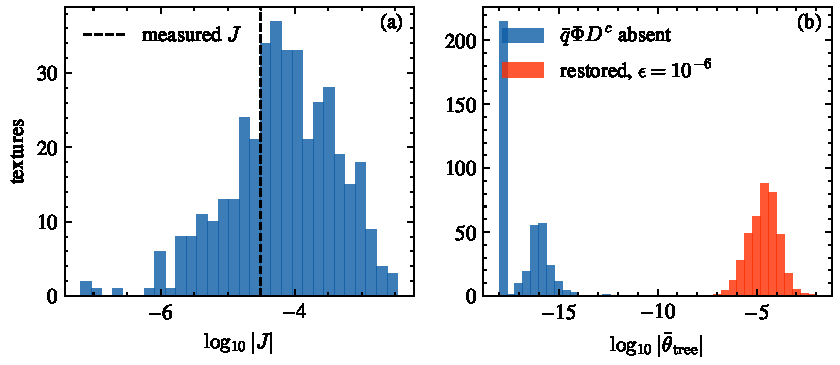
\includegraphics[width=\textwidth]{figures/fig_jarlskog.pdf}
\caption{(a) $|J|$ for $400$ random Froggatt--Nielsen textures with the
texture of Eq.~\eqref{eq:NB} and two CP-breaking doublets; the measured
value is dashed. (b) The tree-level $\bt$ of the same textures, at
machine precision, and with the forbidden links $q_i$--$D^c$ restored
at $\epsilon=10^{-6}$.}
\label{fig:jarlskog}
\end{figure}

To see both effects at once we drew $400$ real textures
$m_{ij}=c_{ij}\lambda^{a_i+a_j}$, with $\lambda=0.225$, charges
$(2,1,0)$ for the down sector and $(4,2,0)$ for the up sector, random
signs and $|c_{ij}|$ log-uniform in $[\tfrac12,2]$, normalized to
$m_b=2.9$~GeV and $m_t=173$~GeV, together with a random complex bridge
of size $|B|=\mu$ (Appendix~\ref{app:numerics}). The textures reproduce
the quark spectrum only to within factors of a few, by construction;
the CP violation is not put in. The determinant is real to
$|\Im\det\mathcal M|/|\det\mathcal M|<2\times10^{-13}$ in every draw,
while $|J|$ has median $7.4\times10^{-5}$ and $10$--$90\%$ range
$5\times10^{-6}$ to $7\times10^{-4}$, with the measured
$J=3.08\times10^{-5}$~\cite{ParticleDataGroup:2024cfk} at the $30$th
percentile (Fig.~\ref{fig:jarlskog}). With a single doublet, $|J|$ is
zero to numerical precision. Restoring the forbidden links at
$\epsilon=10^{-6}$ moves $\bt_{\rm tree}$ to $\sim\epsilon$, which is
the size of the protection the zero provides.

\subsection{The bidoublet vacuum}
\label{sec:bidoublet}

The bidoublet has two neutral VEVs, $\kappa_1$ and $\kappa_2e^{i\alpha}$,
and gives $M_u=\kappa_1(h+\tilde h\,\bar z)$ and $M_d=\kappa_1(hz+\tilde h)$
with $z\equiv(\kappa_2/\kappa_1)e^{i\alpha}$, real $h,\tilde h$
multiplying $\Phi$ and $\tilde\Phi=\sigma_2\Phi^*\sigma_2$. A relative
phase feeds Eq.~\eqref{eq:bartheta} directly: to first order in
$y\equiv\Im z$, and writing $x\equiv\Re z$,
\begin{equation}
  \bt_{\rm tree}=c\,\Im z,\qquad
  c=\frac{\Tr(M_d^{-1}M_u)-\Tr(M_u^{-1}M_d)}{1-x^2},
  \label{eq:kappaphase}
\end{equation}
which for the random textures of Sec.~\ref{sec:layer2} has median
$|c|\simeq45$ at $x=0$ and a $10$--$90\%$ range of $9$ to $300$, dominated
by $m_t/m_b$. So the question is what fixes $\Im z$, and the answer
comes from minimizing the potential.

With all couplings real, every term linear in $\Tr(\Phi^\dagger\tilde\Phi)$
has a real coefficient---$\mu_2^2$, $\lambda_4\Tr(\Phi^\dagger\Phi)$,
$\alpha_2\Tr(\Delta_R^\dagger\Delta_R)$ and the diagonal portals
$g_{aa}\,\chi_a^\dagger\chi_a$---except the off-diagonal portal to the
two CP-breaking doublets,
\begin{equation}
  g_{ab}\,\chi^{(a)\dagger}_R\big(\Phi^\dagger\tilde\Phi\big)\chi^{(b)}_R+{\rm h.c.},
  \qquad g_{ab}\in\mathbb R ,
  \label{eq:portal}
\end{equation}
whose vacuum value is $2\kappa_1\kappa_2\,g_{ab}w_aw_b\cos(\alpha+\theta_a-\theta_b)$.
Summed over $a,b$ the symmetric part of $g$ gives
$4g^S\kappa_1\kappa_2w_1w_2\cos\alpha\cos\varphi$ and the antisymmetric
part $g^A=\tfrac12(g_{12}-g_{21})$ gives
$4g^A\kappa_1\kappa_2w_1w_2\sin\alpha\sin\varphi$; the latter is the only
term in the renormalizable potential that is odd in $\sin\alpha$. Writing
$\kappa_2e^{i\alpha}=X+iY$, the potential is a quadratic form in $(X,Y)$
plus quartics suppressed by $\kappa^2/v_R^2$, with $Y$ entering only
through $D\,Y^2+4g^Aw_1w_2\sin\varphi\,\kappa_1Y$, where
$D\simeq\alpha_3v_R^2+\dots$ is the mass squared of the heavy doublet
direction of the bidoublet. The minimum is therefore
\begin{equation}
  \Im z=\frac{\kappa_2}{\kappa_1}\sin\alpha
  =-\,\frac{2g^A\,w_1w_2\sin\varphi}{D},
  \qquad D=\Ord(\alpha_3v_R^2),
  \label{eq:imz}
\end{equation}
independently of $\mu_2^2$, $\alpha_2$ and $\lambda_4$, which only set
$\Re z=\Ord(1)$. We verified Eq.~\eqref{eq:imz} by minimizing the full
potential at $60$-digit precision, with the light doublet tuned to the
electroweak scale and random order-one couplings: the numerical
$\Im z$ agrees with Eq.~\eqref{eq:imz} to twelve digits, and the
bidoublet sector has no CP-violating minimum of its own unless $D$ is
tuned below $8|\lambda_2|\kappa_1\kappa_2$. Combining with
Eq.~\eqref{eq:kappaphase},
\begin{equation}
  \bt_{\rm tree}\simeq \frac{2c\,g^A}{\alpha_3}\,
  \frac{\vev{\chi_R}^2}{v_R^2}\,\sin\varphi
  \;\approx\;10^{2}\,\frac{g^A}{\alpha_3}
  \Big(\frac{\vev{\chi_R}}{v_R}\Big)^{2}
  \label{eq:bidoubletleak}
\end{equation}
for $w_1=w_2=\vev{\chi_R}$ and $\varphi=\pi/2$. With $v_R\sim10^{15}$~GeV
from the seesaw, $\bt<10^{-10}$ requires
$\vev{\chi_R}\lesssim10^{9}\,(\alpha_3/g^A)^{1/2}$~GeV---the same window
as Eq.~\eqref{eq:window}. The bidoublet is thus relatively real to the
required accuracy because the CP-breaking scale lies six orders of
magnitude below the $\SU(2)_R$ scale; no additional assumption is
needed, and the hierarchy between the two scales, which the seesaw and
the quality bound each impose separately, is now also required by the
bidoublet. If the scalar potential is symmetric under the exchange of
the two doublets (Sec.~\ref{sec:quantization}), $g^A$ vanishes at tree
level and the residual phase is smaller still.

\subsection{Below the $\SU(2)_R$ scale: matter parity and its quality}
\label{sec:layer3}

We break $\SU(2)_R\times\U(1)_{B-L}$ with a triplet $\Delta_R$ of
$B-L=+2$, whose neutral component has $T_{3R}=-1$ and $Y=0$. Integer
isospin makes it center-even, so $\vev{\Delta_R}$ leaves the center
unbroken and the zero is protected below the breaking scale by a
discrete gauge symmetry~\cite{krauss_1989:PRL}. Writing the center
element as $e^{2\pi iT_{3R}}=e^{i\pi Y}e^{-i\pi(B-L)}$ and composing
with elements of the unbroken $\U(1)_Y$ and of the color center, one
finds that on every field of the model
\begin{equation}
  \PR\ \simeq\ (-1)^{3(B-L)} ,
  \label{eq:matterparity}
\end{equation}
odd on quarks, leptons and $\chi_R$, even on $\Phi$, $\Delta_R$ and $D$.
The residual symmetry is matter parity~\cite{Ibanez:1991hv,Martin:1992mq},
and it is genuinely disconnected from the SM gauge group, since it is
$-1$ on $\nu_R$ where $\U(1)_Y\times\SU(3)_C$ can only act trivially.
In this form it is clear that the electroweak VEV ($B-L=0$) leaves it
alone and that $\vev{\chi_R}$ ($B-L=-1$) breaks it, at the scale where
CP is broken. The triplet doubles as the source of right-handed
neutrino masses through $\bar\nu_R^{\,c}\nu_R\Delta_R$; with
$m_\nu\simeq y_\nu^2v^2/(2M_R)$ and $m_\nu\simeq0.05$~eV, $M_R\sim10^{15}$~GeV
for $y_\nu=\Ord(1)$. No other $\Z_2$ built from the available charges,
$(-1)^{2T_{3R}}f(B-L)$ with $f(0)=1$, can make the bidoublet even.

Gravity can still generate gauge-invariant operators that involve the
condensates. We normalize them to $\MPl=1.22\times10^{19}$~GeV; a
mediator of mass $\Lambda<\MPl$ tightens everything below by
$\MPl/\Lambda$. The leading one is
\begin{equation}
  \Ord_5=\frac{\bar q_L\,\Phi\,\chi_R^{(a)\dagger}\,D_R}{\MPl},
\end{equation}
$B-L$ neutral and with two $\SU(2)_R$ doublets; its contribution to
$\bt$ needs two doublets with different phases and vanishes for
$n_\chi=1$. Replacing $\chi_R^\dagger$ by $\chi_R^\dagger\chi_R$
violates $B-L$, but the triplet makes room for
$\bar q_L\Phi\chi_R\Delta_RD_R/\MPl^2$ at dimension six, which feeds
the same entry with an extra $\vev{\Delta_R}/\MPl\sim10^{-4}$ and does
not change the estimate. The dimension-five operator fills the empty
block with $\Delta_{q_LD_R}\sim\vev{\chi^{(a)}}^{*}/\MPl$ times a flavor
matrix, and through $\det\mathcal M=\det m\,(\mu-Bm^{-1}\Delta)$ shifts
\begin{equation}
  \delta\bt\simeq\frac{\Im\big(B\,m^{-1}\Delta\big)}{\mu}
  \sim F\,\frac{\vev{\chi_R}^{2}}{\MPl\,\mu}
  \label{eq:leak}
\end{equation}
when the flavor matrix of $\Ord_5$ is aligned with the down Yukawas, so
that $m^{-1}\Delta$ carries no hierarchy. Requiring $\delta\bt<10^{-10}$
with $|B|\sim\mu$, i.e.\ $\vev{\chi_R}\sim\mu/F$, gives
\begin{equation}
  \vev{\chi_R}\sim\mu\lesssim10^{9}~{\rm GeV}.
  \label{eq:window}
\end{equation}
Figure~\ref{fig:leakage} checks the scaling with the exact
determinant. If the coefficients of $\Ord_5$ are flavor anarchic, the
light-quark entries of $m^{-1}$ enhance the leak by about two orders of
magnitude, and if they are of order one rather than of the size of
$y_b$, by a further $v/m_b\sim60$, bringing the bound down to
$10^{5\text{--}7}$~GeV. Equation~\eqref{eq:window} is thus the
optimistic end of a range set by how much flavor structure the
ultraviolet respects; it is still weaker than the $\sim10^2$~TeV often
quoted for Nelson--Barr models with $\Lambda\sim\MPl$.

\begin{figure}[t]
\centering
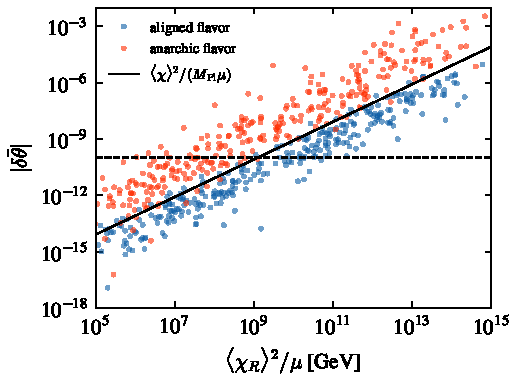
\includegraphics[width=0.6\textwidth]{figures/fig_leakage.pdf}
\caption{Tree-level $|\delta\bt|$ from the dimension-five operator,
computed from the exact determinant for random textures, bridges and
scales, with flavor-aligned and anarchic coefficients. The solid line
is $\vev{\chi_R}^2/(\MPl\mu)$ and the dashed line the bound
$10^{-10}$.}
\label{fig:leakage}
\end{figure}

With the exact texture the one-loop contribution to $\bt$
vanishes~\cite{BENTO199195}. The first loop effect is at two loops,
governed by $\Im(B_i^*B_j)\,(mm^\dagger)_{ij}$ divided by $\mu^2$, and is
of order $(16\pi^2)^{-2}y_b^2y_s^2$, or about
$10^{-15}$~\cite{Dine:2015jga}; a complete
calculation for this texture is left for future work. A vector-like
quark at $10^{8\text{--}9}$~GeV has no observable flavor-changing
effects: its right-handed mixing with light quarks is of order one, but
the left-handed mixing is $\sim m_b|B|/(|B|^2+\mu^2)\lesssim10^{-8}$.
When $\vev{\chi_R}$ breaks the residual $\Z_2$ it makes domain walls, but
since $\pi_0$ of the group left by $\vev{\Delta_R}$ is $\Z_2$, strings form
first and the walls end on them~\cite{kibble_1982:PRD}. Such networks
collapse, and at $\vev{\chi_R}\sim10^{8\text{--}9}$~GeV the walls never
dominate the energy density; primordial black holes offer a further
sink~\cite{Stojkovic:2005zh}. A quantitative treatment of the network
is beyond our scope.

% =========================================================================
\section{The unitarity triangle}
\label{sec:flavor}
% =========================================================================

\subsection{Link diagrams and perfect matchings}

The measured angles~\cite{ParticleDataGroup:2024cfk,UTfit:2022hsi},
\begin{equation}
  \alpha=(91.0\pm2.8)^\circ,\qquad
  \beta=(22.6\pm0.5)^\circ,\qquad
  \gamma=(66.4^{+2.7}_{-2.8})^\circ,
  \label{eq:UTangles}
\end{equation}
with $\alpha$ from unitarity, sit remarkably close to $\pi/2$, $\pi/8$
and $3\pi/8$~\cite{Arkani-Hamed:2026uos}.
Following Ref.~\cite{Arkani-Hamed:2026uos} we draw the Yukawa sector as
a bipartite graph with left-handed nodes $q_i$, $D_L$ and right-handed
nodes $u^c_j$, $d^c_j$, $D^c$; links are nonzero entries and missing
links are texture zeros (Fig.~\ref{fig:linkgraph}). One class of zeros,
the links $q_i$--$D^c$, is now dictated by $\SU(2)_R$.

\begin{figure}[t]
\centering
\begin{tikzpicture}[
   >=stealth,
   nd/.style ={circle,draw,fill=white,inner sep=1.6pt,minimum size=5.5mm,font=\small},
   lk/.style ={thick},
   br/.style ={thick,red!70!black},
   fb/.style ={dashed,thick,gray!60},
   lbl/.style={font=\scriptsize,inner sep=1pt}
  ]
\node[nd] (q1) at (0, 3.0) {$q_1$};
\node[nd] (q2) at (0, 2.0) {$q_2$};
\node[nd] (q3) at (0, 1.0) {$q_3$};
\node[nd] (DL) at (0, 0.0) {$D_L$};
\node[nd] (d1) at (4.2, 3.0) {$d^c_1$};
\node[nd] (d2) at (4.2, 2.0) {$d^c_2$};
\node[nd] (d3) at (4.2, 1.0) {$d^c_3$};
\node[nd] (Dc) at (4.2, 0.0) {$D^c$};
\draw[lk] (q1)--(d1) node[lbl,midway,above]{$m_{11}$};
\draw[lk] (q1)--(d2) node[lbl,pos=.25,above,sloped]{$m_{12}$};
\draw[lk] (q2)--(d2) node[lbl,midway,above]{$m_{22}$};
\draw[lk] (q2)--(d3) node[lbl,pos=.25,above,sloped]{$m_{23}$};
\draw[lk] (q3)--(d3) node[lbl,midway,above]{$m_{33}$};
\draw[br] (DL)--(d2) node[lbl,pos=.75,above,sloped]{$B_2$};
\draw[br] (DL)--(d3) node[lbl,pos=.75,below,sloped]{$B_3e^{i\varphi}$};
\draw[lk] (DL)--(Dc) node[lbl,midway,below]{$\mu$};
\foreach \q in {q1,q2,q3} \draw[fb] (\q)--(Dc);
\node[lbl,gray!70!black,anchor=west] at (4.6,0.0) {$q_i$--$D^c$: no $\SU(2)_R$ invariant};
\end{tikzpicture}
\caption{The down sector of the minimal graph of
Sec.~\ref{sec:minimalgraph}. Black links are real (Yukawas and the
Dirac mass $\mu$), red links are the complex bridges
$B_j=\sum_aF^{(a)}\vev{\chi^{(a)}_R}$, and dashed links are forbidden
by $\SU(2)_R$. With $D^c$ left a single neighbor, every perfect matching
contains $\mu$ and none contains a bridge. The unique cycle
$D_L\to d^c_2\to q_2\to d^c_3\to D_L$ carries the phase
$\varphi=\arg(B_2^*B_3)$.}
\label{fig:linkgraph}
\end{figure}

For an $n\times n$ matrix, $\det Y=\sum_{\pi}\mathrm{sgn}(\pi)\prod_iY_{i\pi(i)}$,
and a permutation contributes only if each factor is a link, that is,
if it is a perfect matching of the graph:
\begin{equation}
  \det Y=\sum_{\text{perfect matchings }M}\pm\prod_{\ell\in M}Y_\ell .
  \label{eq:detmatch}
\end{equation}
Ref.~\cite{Arkani-Hamed:2026uos} uses this through sparsity: a graph
with a single perfect matching has a monomial determinant whose phase
can be moved onto an unused link, which works for $94$ of its $99$
textures. Here the mechanism is different. A matching must cover
$D^c$, whose only link is $\mu$, so it uses $D_L$; every bridge ends on
$D_L$, so no matching contains a bridge. Each term of
Eq.~\eqref{eq:detmatch} is then $\mu$ times a matching of the real $m$,
which is Eq.~\eqref{eq:det} again, and it holds for any $m$, sparse or
dense. Restoring one forbidden link at strength $\epsilon$ adds six
phase-carrying matchings and an imaginary part of order $\epsilon$
(Fig.~\ref{fig:jarlskog}b).

The gauge zero protects $\bt$; further zeros make the triangle
predictive. A connected bipartite graph with $V$ nodes and $L$ links
has $L-V+1$ independent cycles, and since every node can absorb one
phase, a single physical phase needs $L=V$. The nine-node graphs of
Ref.~\cite{Arkani-Hamed:2026uos} have nine links; ours have
$V=3+1+3+3+1=11$ and so eleven links, carrying eleven magnitudes and
one phase. Only $|B|/\mu$ is visible at low energy, and if the two
doublets, which carry identical charges, are exchanged by a symmetry
of the scalar potential, then
\begin{equation}
  |B_2|=|B_3|,
  \label{eq:equalvevs}
\end{equation}
leaving ten magnitudes for ten observables and the phase as a
prediction. On the cycle of Fig.~\ref{fig:linkgraph} the rephasing
invariant is
\begin{equation}
  \varphi=\arg\!\big(m_{22}B_2^{*}B_3m_{23}^{*}\big)=\arg\!\big(B_2^{*}B_3\big),
  \label{eq:phivev}
\end{equation}
the relative phase of the two doublet VEVs. The ``Yukawa triangle'' of
Ref.~\cite{Arkani-Hamed:2026uos} is drawn by two VEVs: isosceles by
Eq.~\eqref{eq:equalvevs}, with apex angle $\varphi$, and its shape is a
question about a scalar potential.

\subsection{The minimal graph}
\label{sec:minimalgraph}

The simplest connected eleven-link graph with one cycle and the
observed hierarchies is
\begin{equation}
  Y_u=\mathrm{diag}(u_{11},u_{22},u_{33}),
  \qquad
  m=\begin{pmatrix}
      m_{11}&m_{12}&0\\
      0&m_{22}&m_{23}\\
      0&0&m_{33}
    \end{pmatrix},
  \qquad
  B=(0,\,b,\,b\,e^{i\varphi}),
  \label{eq:minimal}
\end{equation}
plus $\mu$. With $Y_u$ diagonal the whole CKM matrix comes from
$H_{\rm eff}$, and the six parameters
$(m_{11},m_{12},m_{22},m_{23},m_{33},b/\mu)$ are fixed by the three
down-type masses and $|V_{us}|,|V_{cb}|,|V_{ub}|$ (at $M_Z$). These
equations have two exact solutions. One gives
\begin{equation}
  (\alpha,\beta,\gamma)=(90.11^\circ,\,23.89^\circ,\,65.99^\circ)
  \qquad\text{at }\varphi=\pi/2,
  \label{eq:prediction}
\end{equation}
with $|B|/\mu=2.0$, the order-one ratio that Sec.~\ref{sec:layer2}
needs and that the fit was not asked for; the other gives
$(43.5^\circ,16.2^\circ,120.3^\circ)$ and is excluded by the measured
$\alpha$ and $\gamma$. Following both as $\varphi$ varies
(Fig.~\ref{fig:alphaphi}), the first obeys $\alpha=\varphi$ to within
$0.11^\circ$ over $\varphi\in[\pi/8,5\pi/8]$, so in this texture the
VEV phase \emph{is} the angle $\alpha$, which is the locking mechanism of
Ref.~\cite{Arkani-Hamed:2026uos} realized by a scalar potential.

\begin{figure}[t]
\centering
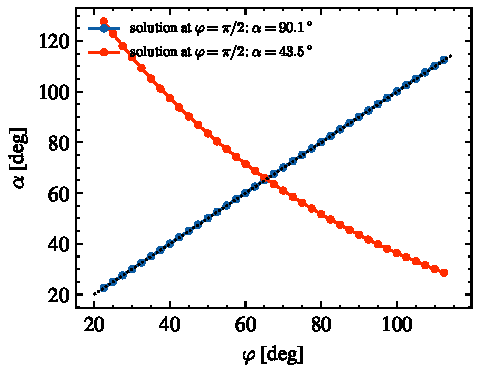
\includegraphics[width=0.55\textwidth]{figures/fig_alpha_phi.pdf}
\caption{The angle $\alpha$ for the two exact solutions of the minimal
graph, Eq.~\eqref{eq:minimal}, followed as the bridge phase $\varphi$
varies. One branch tracks $\alpha=\varphi$ (dotted) to within
$0.11^\circ$.}
\label{fig:alphaphi}
\end{figure}

Against the data, Eq.~\eqref{eq:prediction} pulls by $-0.3\sigma$ in
$\alpha$, $-0.1\sigma$ in $\gamma$ and $+2.6\sigma$ in $\beta$. The
last number is not the graph's doing. For any triangle the law of sines
gives
\begin{equation}
  \sin\beta = R_b\,\sin\alpha,
  \qquad
  R_b=\left|\frac{V_{ud}V_{ub}}{V_{cd}V_{cb}}\right| ,
  \label{eq:sinbeta}
\end{equation}
so once a texture fixes $\alpha=90^\circ$ and reproduces $|V_{ub}|$ and
$|V_{cb}|$, the value $\beta=\arcsin R_b$ is forced, and it is also the
largest $\beta$ available at these magnitudes (Fig.~\ref{fig:betadelta}).
With the average $|V_{ub}|=3.82\times10^{-3}$ this is $23.89^\circ$; with
the exclusive $3.70\times10^{-3}$ it is $23.10^\circ$, a $1.0\sigma$ pull;
with $3.60\times10^{-3}$ it is $22.44^\circ$. The tension is the
long-standing $|V_{ub}|$ puzzle~\cite{ParticleDataGroup:2024cfk,Bernlochner:2011uc,Belle:2023asx}
seen through the triangle. LHCb is projected to measure $\beta$ to
$0.2^\circ$ with $50~{\rm fb}^{-1}$ and $0.08^\circ$ with
$300~{\rm fb}^{-1}$~\cite{Arkani-Hamed:2026uos}, so together with a
settled $|V_{ub}|$ the relation $\alpha=\pi/2$ will be tested sharply.

\begin{figure}[t]
\centering
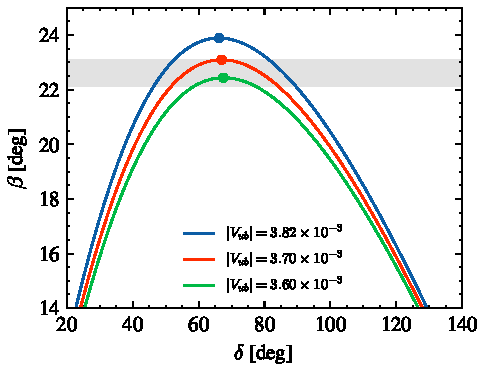
\includegraphics[width=0.55\textwidth]{figures/fig_beta_delta.pdf}
\caption{$\beta$ as a function of the CKM phase $\delta$ at fixed
$|V_{us}|$, $|V_{cb}|$ and three values of $|V_{ub}|$. Dots mark
$\alpha=90^\circ$, which coincides with the maximum of each curve,
Eq.~\eqref{eq:sinbeta}. The band is the measured $\beta$.}
\label{fig:betadelta}
\end{figure}

\subsection{All eleven-link graphs}
\label{sec:scan}

Equation~\eqref{eq:minimal} was chosen by hand, so we enumerated the
whole family. The admissible links are $q_i$--$u^c_j$, $q_i$--$d^c_j$,
the bridges $D_L$--$d^c_j$ and the mandatory $D_L$--$D^c$, with the
$q_i$--$D^c$ links absent. Requiring that $Y_u$ and $m$ each have a
perfect matching (no massless quark), that the graph be connected with
eleven links, and that it contain at least two bridges, the graph
version of $n_\chi\ge2$, leaves $6696$ graphs ($26{,}352$ without the
bridge condition), which fall into $34$ classes under
$S_3^{(q)}\times S_3^{(u^c)}\times S_3^{(d^c)}$:
$(n_u,n_m,n_B)=(4,4,2)$ for $16$, $(3,5,2)$ and $(5,3,2)$ for $8$ each,
and $(3,4,3)$, $(4,3,3)$ for one each. A third bridge spends a link that
the two matchings and connectivity would otherwise need, which is why
so few classes have one.

For each class we solved the nine magnitude equations (six masses and
$|V_{us}|,|V_{cb}|,|V_{ub}|$ at $M_Z$) at $\varphi=\pi/2$ with equal bridge
moduli, from several hundred random starting points, and kept every
distinct exact solution; since magnitudes cannot tell $V$ from $V^*$,
solutions are folded onto $J>0$. Twelve classes have no exact solution,\footnote{Two of them come
within a relative $10^{-4}$ of one, on branches A and B below; at the
precision of the input masses they would count as fits, and they do
not change any conclusion.}
five have only CP-conserving ones, and seventeen have CP-violating
solutions, usually more than one. Across the family these solutions
land on just four points in the $(\alpha,\beta,\gamma)$ plane
(Fig.~\ref{fig:classes}):
\begin{equation*}
\begin{array}{lccc}
 & \alpha & \beta & \gamma \\
\text{A (11 classes)} & 88.7^\circ\text{--}90.1^\circ & 23.89^\circ & 66.0^\circ\text{--}67.4^\circ\\
\text{B (5 classes)}  & 66.9^\circ\text{--}68.0^\circ & 21.9^\circ\text{--}22.1^\circ & 90.0^\circ\text{--}91.2^\circ\\
\text{C (4 classes)}  & 60.9^\circ\text{--}62.0^\circ & 20.7^\circ\text{--}21.0^\circ & 97.1^\circ\text{--}98.3^\circ\\
\text{D (4 classes)}  & 43.5^\circ\text{--}44.1^\circ & 16.2^\circ\text{--}16.4^\circ & 119.6^\circ\text{--}120.3^\circ
\end{array}
\end{equation*}
On branch A the phase locks $\alpha$, on branch B it locks $\gamma$,
and on C and D it locks neither. Only A is compatible with the measured
$\alpha$ and $\gamma$; B misses $\alpha$ by $8\sigma$, and C and D by
more. The minimal graph belongs to A and is its best fit. The robust
statement is therefore that every eleven-link texture consistent with
the measured angles has $\alpha\simeq\varphi$, with $\beta$ then given by
Eq.~\eqref{eq:sinbeta}.

\begin{figure}[t]
\centering
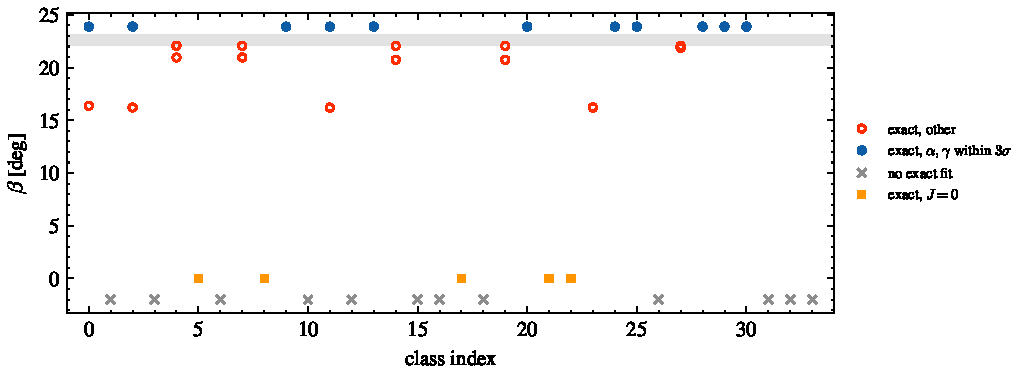
\includegraphics[width=\textwidth]{figures/fig_classes.pdf}
\caption{Exact solutions of the nine magnitude equations for each of
the $34$ eleven-link classes at $\varphi=\pi/2$. A class can have several
solutions. Filled circles have $\alpha$ and $\gamma$ within $3\sigma$
of the data; open circles do not; squares are CP-conserving solutions
($\beta=0$); crosses mark classes with no exact solution. The band is
the measured $\beta$.}
\label{fig:classes}
\end{figure}

\subsection{Without the vector-like quark}
\label{sec:noD}

Removing $D_L$ and $D^c$ leaves nine nodes and nine links, exactly the
setting of Ref.~\cite{Arkani-Hamed:2026uos}. Handing our fitting code
their Example~I, with $Y_u$ nonzero at $(12)$, $(21)$, $(22)$, $(33)$, $m$
nonzero at $(12)$, $(21)$, $(22)$, $(23)$, $(33)$ and the phase $\pi/2$ on
$Y^u_{12}$, returns $\alpha=88.92^\circ$, $\beta=23.89^\circ$ and
$\gamma=67.19^\circ$, inside
their $\varphi=\pi/2$ cluster $[88.74^\circ,90.03^\circ]$ and between
their classes at $88.914^\circ$ and $88.957^\circ$, together with a
second exact solution near branch D. Its $\beta$ is again
$\arcsin R_b$: their region~I sits at $\beta\simeq23.65^\circ$--$23.95^\circ$,
while their $\varphi=\pi/8$ classes reach $\beta\simeq22.5^\circ$ at
$\delta\simeq85^\circ$, a different point on the same curve
(Fig.~\ref{fig:betadelta}), possible because those classes do not fit
all three magnitudes at once. The two frameworks overlap in $\alpha$:
our branch A spans $88.7^\circ$--$90.1^\circ$, just reaching past the
upper edge of their $\varphi=\pi/2$ islands, and the nearest of their
classes, with $\alpha=90.028^\circ$, $\beta=22.683^\circ$ and
$\gamma=66.253^\circ$, differs from
Eq.~\eqref{eq:prediction} by $1.2^\circ$ in $\beta$. What separates them
is how each treats $|V_{ub}|$, and the comparison should be revisited
once that determination settles.

Without $D$, the parity has nothing to do. Every one of the eighteen
SM Yukawa links $q$--$u^c$ and $q$--$d^c$ is $\PR$-even; no node is
isolated, the reality of $\det Y$ has to be checked texture by
texture, the Nelson--Barr block disappears, and the CP phase must sit
in a Yukawa coupling, where ultraviolet CP no longer protects $\bt$.
The vector-like quark is what makes the parity bite, what protects
$\bt$, and what moves the textures off the nine-link islands. Dense
textures, in turn, predict nothing: with the Froggatt--Nielsen matrices
of Sec.~\ref{sec:layer2} and the same bridge at $\varphi=\pi/2$, the
central $68\%$ of $\alpha$ spans $1^\circ$--$176^\circ$, in line with the
finding of Ref.~\cite{Arkani-Hamed:2026uos} that at least four zeros
are needed for a robust angle--phase relation. The parity supplies one
of them; the rest of Eq.~\eqref{eq:minimal} is input.

\subsection{Why $\pi/2$, and why not $\pi/8$}
\label{sec:quantization}

The phases of the $\chi_R$ VEVs are fixed by the $\chi$ sector of the
potential, and here the gauge charges force a term that the discussion
so far has not used: $\chi_R$ carries exactly the quantum numbers of
the right-handed lepton doublet, so the scalar analogue of the seesaw
coupling,
\begin{equation}
  h_{ab}\,\chi^{(a)T}_R\,i\sigma_2\,\Delta_R\,\chi^{(b)}_R+{\rm h.c.},
  \label{eq:cubic}
\end{equation}
is allowed by every symmetry of the model ($B-L$: $-1-1+2=0$; center:
$(-)(-)(+)=+$). It is cubic, and with $\vev{\Delta_R}=v_R$ it contributes
$v_R w^2[h_{11}\cos2\theta_1+h_{22}\cos2\theta_2+2h_{12}\cos(\theta_1+\theta_2)]$,
which dominates the phase-dependent quartics
$m_{12}^2w^2\cos\varphi$ and $\lambda_5w^4\cos2\varphi$ by $v_R/w\sim10^6$
unless $h_{ab}$ is absurdly small. The phases are therefore set by
Eq.~\eqref{eq:cubic}, and the outcome depends on the symmetry of the
$\chi$ sector:
\begin{itemize}
\item Under a plain exchange $\chi_1\leftrightarrow\chi_2$, $h_{11}=h_{22}$,
  and the minimum has $\varphi\in\{0,\pi\}$: the two VEVs are relatively
  real and the model has no CP violation at all. The exchange symmetry
  that makes $|B_2|=|B_3|$ natural is therefore not an option by
  itself.
\item Under the twisted exchange $E:\ \chi_1\to-i\chi_2,\ \chi_2\to-i\chi_1$,
  a $\Z_4$ with $E^2:\chi_a\to-\chi_a$, one has $h_{22}=-h_{11}$ and
  $h_{12}=0$, while $|\chi_1|^2\leftrightarrow|\chi_2|^2$ still forces
  $w_1=w_2$. The cubic term becomes
  $-2h\,v_Rw^2\sin(\theta_1+\theta_2)\sin(\theta_1-\theta_2)$, whose
  minimization in $\theta_1-\theta_2$ gives $\cos\varphi=0$ exactly, for
  either sign of $h$ and independently of $\theta_1+\theta_2$:
  \begin{equation}
    \varphi=\pm\frac{\pi}{2},
    \label{eq:phiquant}
  \end{equation}
  shifted only by $m_{12}^2/(2hv_R)\lesssim10^{-6}$ from the subleading
  quartics. The two signs are the CP-conjugate vacua of
  Sec.~\ref{sec:scan}.
\item With no symmetry, $h_{11}h_{22}<0$ gives $|\varphi|$ within a few
  degrees of $\pi/2$ and $h_{11}h_{22}>0$ gives $\varphi\in\{0,\pi\}$.
\end{itemize}
A $\Z_4$ acting on the two phase words thus yields $\varphi=\pi/2$ from
the potential itself, with the $\Z_4$ root of unity entering through
$E^2=-1$ rather than through a larger gauge group; the Pati--Salam
$\SU(4)_C$ center remains a possible gauge origin for $E$ but is not
needed for the result. $E$ is a symmetry of the scalar potential; the
bridge couplings break it, as they must, since an $E$-invariant bridge
would give every $B_j$ the same phase. The bridges couple $\chi_1$ and
$\chi_2$ to orthogonal flavor directions, so they do not regenerate
$h_{12}$ or the $\chi_1^\dagger\chi_2$ mass mixing at one loop, and a
mild violation of $E$ shifts $\varphi$ by a small amount that does not
touch $\bt$, which is protected by the gauge parity alone.

The same logic stops short of $\beta\simeq\pi/8$, which
Ref.~\cite{Arkani-Hamed:2026uos} obtains from a $\Z_8$ acting on flavons
through
\begin{equation}
  \frac{z_1-z_2}{z_1+z_2}=-i\tan\frac{\theta}{2},
  \qquad |z_1|=|z_2|,\ \ \theta=\arg(z_2/z_1),
  \label{eq:bisect}
\end{equation}
since no cubic or quartic invariant of two doublets quantizes a relative
phase to $\pi/8$. The potential accounts for $\alpha\simeq\pi/2$; $\beta$
is left to $|V_{ub}/V_{cb}|$.

\subsection{An axion instead?}

The mechanism needs no axion, but the structure tolerates one. A
Peccei--Quinn axion at $f_a\sim10^{15}$~GeV would need PQ-violating
operators suppressed up to dimension $d\gtrsim23$ for order-one
Planck-normalized coefficients, and the center parity removes only
half of them. Its mass would be
\begin{equation}
  m_a\simeq\frac{f_\pi m_\pi}{f_a}\frac{\sqrt{m_um_d}}{m_u+m_d}
  \approx 5.7~{\rm neV}\,\frac{10^{15}~{\rm GeV}}{f_a},
  \label{eq:ma}
\end{equation}
in the range of DMRadio and CASPEr~\cite{dmradio,casper}. The two
options are cleanly distinguishable: the Nelson--Barr route predicts
no axion and a CP-breaking sector at or below $10^9$~GeV.

% =========================================================================
\section{Conclusions}
\label{sec:conclusions}
% =========================================================================

The discrete symmetry that Nelson--Barr models introduce by hand can
be part of the gauge group, and the SM hypercharges point to which
one. In the left-right completion, an $\SU(2)_R$-singlet vector-like
quark cannot couple to the quark doublets through the bidoublet, the
Bento--Branco--Parada texture follows, and $\arg\det\mathcal M=0$ holds
for every texture while the CKM phase stays generic: over $400$ random
textures the measured Jarlskog invariant lands at the $30$th
percentile. The protecting symmetry is the center of $\SU(2)_R$, which
survives the triplet that breaks $\SU(2)_R$ and sets the seesaw scale,
and which below that scale is matter parity. Its quality is fixed by a
dimension-five operator and puts the CP-breaking sector below
$10^9$~GeV, lower if the ultraviolet does not respect flavor. The
bidoublet vacuum is relatively real to the required accuracy as a
consequence of the potential: its only CP-odd tadpole is a portal to the
two CP-breaking doublets, suppressed by
$(\vev{\chi_R}/v_R)^2\sim10^{-12}$--$10^{-14}$, which bounds the
CP-breaking scale by the same $10^9$~GeV as the quality argument. The
cubic coupling of the doublets to the triplet fixes their relative phase,
and a $\Z_4$ exchange symmetry of the potential sets it to $\pi/2$
exactly.

In the language of link diagrams the gauge zero removes every
phase-carrying perfect matching at once, and the one physical phase
becomes the relative phase of two VEVs. Among all $6696$ eleven-link
graphs, the solutions compatible with the measured angles lie on a
single branch on which that phase is the angle $\alpha$. The value
$\varphi=\pi/2$ selected by the $\Z_4$ then gives $(90^\circ,23.9^\circ,66^\circ)$, with $\beta$
determined by $R_b$, so the construction will be tested by the LHCb
measurement of $\beta$ together with the resolution of $|V_{ub}|$, and,
independently of flavor, by the absence of an axion.

\section*{Acknowledgements}
D.\v{S}.\ and D.S.\ are partially supported by the US National Science
Foundation under Grant No.\ PHY-2310363.

\paragraph{Disclosure of generative AI use}
Claude (Anthropic) was used to improve the text and to assist in
writing the numerical code. The authors have verified all derivations,
numerical results and references, and take full responsibility for the
content.

\paragraph{Author contributions}
Both authors contributed equally to all aspects of this work.

\paragraph{Funding information}
US National Science Foundation, Grant No.\ PHY-2310363.

\paragraph{Code availability}
The Python code that produces every number and figure in this paper
is provided with the submission.

\begin{appendix}
\numberwithin{equation}{section}

\section{Registers in components}
\label{app:registers}

With $\ket1,\ket2,\ket3=\ket r,\ket g,\ket b$, the color generators in
matrix units are
\begin{align}
  \lambda_1&=e_{12}+e_{21}, &
  \lambda_2&=i(e_{21}-e_{12}), &
  \lambda_3&=e_{11}-e_{22}, &
  \lambda_4&=e_{13}+e_{31}, \notag\\
  \lambda_5&=i(e_{31}-e_{13}), &
  \lambda_6&=e_{23}+e_{32}, &
  \lambda_7&=i(e_{32}-e_{23}), &
  \lambda_8&=\tfrac{1}{\sqrt3}(e_{11}+e_{22}-2e_{33}).
\end{align}
The raising operators $e_{12}$, $e_{13}$, $e_{23}$ and their conjugates
are the six charged gluon vertices; $e_{12}$, for instance, turns a green
quark red. $\lambda_3$ weighs $r$ against $g$ and $\lambda_8$ weighs
$r,g$ against $b$, the two Cartan generators of a rank-two algebra.

In the same language $u_R$ carries $n_1=+4$ unary indices, $e_R$ carries
six anti-indices and $\nu_R$ none. On the binary state
$\ket{0110}=\ket{d_Lu_Lu_Ld_L}$, $\sigma^+$ acting on the first slot gives
$\ket{1110}$ and on the second gives zero, the nilpotency of the
raising operator in the fundamental representation; a $W^+$ vertex is
such a single-slot substitution. On $\ket{132}=\ket{rbg}$, $e_{23}$ acting
on the second slot gives $\ket{rgg}$. Of the six orderings of $rgb$,
only $\tfrac1{\sqrt6}\varepsilon_{ijk}\ket{ijk}$ is invariant, picking up
$\det U=1$: color neutrality belongs to the combination, not to any
single ordering.

\section{Numerical procedure}
\label{app:numerics}

All numbers and figures are produced by the short Python scripts
provided with the submission. The inputs are $\overline{\rm MS}$ masses at $M_Z$ and CKM magnitudes~\cite{ParticleDataGroup:2024cfk},
\begin{equation}
  (m_u,m_c,m_t)=(0.0013,\,0.62,\,172)~{\rm GeV},\quad
  (m_d,m_s,m_b)=(0.0028,\,0.055,\,2.89)~{\rm GeV},
\end{equation}
with $|V_{us}|=0.2243$, $|V_{cb}|=0.0410$ and $|V_{ub}|=0.00382$.

\paragraph{Random textures.} Real matrices $m_{ij}=c_{ij}\lambda^{a_i+a_j}$
with $a=(2,1,0)$ (down) and $(4,2,0)$ (up), $c_{ij}$ of random sign with
$|c_{ij}|$ log-uniform in $[\tfrac12,2]$ (CP requires real, not
positive, couplings), are scaled so that their largest singular values
are $2.9$ and $173$~GeV. The bridge is $B_i\propto r_i+ir_i'$ with standard
normal $r_i,r_i'$ and $|B|=\mu$; for the one-doublet control all $B_i$
share a phase. The CKM matrix follows from diagonalizing $H_{\rm eff}$
and $m_um_u^\dagger$. Median singular values are $(0.011,0.18,2.9)$~GeV
for $m$ and $(0.0019,0.47,173)$~GeV for $m_u$, within a factor of four
of the measured masses. The coefficient $c$ of
Eq.~\eqref{eq:kappaphase} is evaluated on the same textures as
$\Tr(M_d^{-1}M_u)-\Tr(M_u^{-1}M_d)$; it agrees with the finite-difference
derivative of $\arg\det(M_uM_d)$ with respect to $\Im z$ once the
$\bt=\pi$ branch of sign-flipped determinants is removed, and has median
$45$ and $10$--$90\%$ range $9$ to $300$.

\paragraph{Leakage.} For Fig.~\ref{fig:leakage}, $\mu$ is log-uniform in
$[10^4,10^{13}]$~GeV, $F$ log-uniform in $[0.1,1]$ and
$|\vev{\chi_R}|=\mu/F$, with two doublets of random relative phase.
The dimension-five entry is $\Delta=m\,k\,\vev{\chi}^*/\MPl$ in the aligned
case and $\Delta=m_b\,k\,\vev{\chi}^*/\MPl$ in the anarchic one, with
$k$ standard normal. The phase is computed from the Schur complement
$\mu-Bm^{-1}\Delta$, since a direct $4\times4$ determinant loses all
precision at $\mu/m_d\sim10^{15}$. The median of
$|\delta\bt|\,\MPl\mu/\vev{\chi_R}^2$ is $0.18$ (aligned) and $22$
(anarchic).

\paragraph{Potential minimization.} For Eq.~\eqref{eq:imz} the full
bidoublet potential, including all quartics and the portals
\eqref{eq:portal}, is minimized in $(\kappa_1,X,Y)$ with $60$-digit
arithmetic, the light eigenvalue of the $(\kappa_1,\kappa_2)$ mass matrix
tuned to $-(100~{\rm GeV})^2$, for random couplings with $\mu_2^2$ of order
$v_R^2$; the Hessian is checked to be positive. For
Eq.~\eqref{eq:phiquant} the $\chi$-sector phase potential, including the
cubic term \eqref{eq:cubic}, $m_{12}^2$, $\lambda_5$ and $\lambda_6$, is
minimized from random starts under each symmetry choice.

\paragraph{Graph scan.} \texttt{scan.py} enumerates the graphs, reduces
them to classes by brute-force canonical forms under
$S_3^3$, and for each class runs bounded least squares on the
logarithms of the nine observables from $500$ random starts. A
solution is kept if the sum of squared log-residuals is below
$10^{-16}$, and solutions are grouped by their angles to $0.1^\circ$. The
phase sits on a bridge on the graph's cycle; if no bridge lies on the
cycle, the phase is unphysical and the solutions are CP-conserving.

\end{appendix}

\bibliography{refs}

\nolinenumbers

\end{document}
